\documentclass[10pt]{article}

\usepackage{lipsum}
\usepackage{url}
\usepackage{float}
\usepackage{amsmath}
\usepackage{enumitem}
\usepackage{graphicx}
\usepackage{caption}
\usepackage{subcaption}
\usepackage{rotating}
\usepackage{geometry}
\usepackage{listings}
\usepackage{hyperref}
\usepackage[T1]{fontenc}
\usepackage[numbered]{matlab-prettifier}

\newcommand{\documentTitle}{Lab 4 - Signal Processing II: Active Circuits}
\newcommand{\documentAuthor}{Andrew Pham, Aneel Damaraju}
\newcommand{\courseTitle}{ELEC 240}
\newcommand{\testDate}{September 26, 2018}
\newcommand{\reportDate}{October 2, 2018}

\geometry{margin=1in}
\lstset{
    tabsize=4,
    basicstyle={\ttfamily},
    captionpos=b,
    belowskip=1em,
    aboveskip=1em,
    numbers=left,
	escapechar=\@,
}

\title{
    \textbf{\courseTitle} \\
    \textbf{\documentTitle} \\
    \bigskip
    \textbf{\large{Test performed: \testDate}} \\
    \textbf{\large{Report submitted: \reportDate}} \\
    \bigskip
    \bigskip
}
\author{\documentAuthor}
\date{}

\begin{document}

\maketitle

\newpage

\section{Objective}

Your text here

\medskip

\textit{Note (To be deleted): Think of this test report as a document with your peers as your readers. This means you can assume a similar knowledge background as you. Your readers should be able to easily understand what is going on, and also be able to repeat your lab results based on your document and all references you cite.}

\textit{For the Objective section, identify the test you performed and its objectives. The objectives of the test are important to state because they are usually analyzed in the conclusion to determine whether the test succeeded.}

\section{Materials}

Your text here

\medskip

\textit{Note (To be deleted): Provide a bullet point list of components, software tools, and hardware (such as the NI VirtualBench or DMM) used during the lab}

\section{Test Description}

Your text here

\medskip

\textit{Note (To be deleted): This section provides a summary of the test your team performed. Give enough information so readers can understand what you did, but do not go into the details of every step.}

\subsection{Pre-Lab Calculations and Schematics}

Your text here

\medskip

\textit{Note (To be deleted): Include the homework pre-calculations and schematics that serve as the initial setup for the test. Briefly explain the importance of each item you include. You may want to number your equations/figures so you can refer to them in later sections. Including photos of handwritten work is okay.}

\section{Results and Discussion}

\qquad After setting up the Op-Amp into an open-loop response configuration in Part A for Experiment 4.1, we produced a 2 $V_{pp}$, 20 Hz sine wave. We measured the voltage output from the Op-Amp and observed a max voltage of 14.4 V and a minimum voltage of -13.6 V. We then connected a 100 $\Omega$ resistor between $v_{OUT}$ and ground. This caused the voltage to drop dramatically because the resistor itself has a significant voltage drop. We now observed a max voltage of 3.12 V and a minimum voltage of -1.64 V. After removing the 100 $\Omega$ resistor, we set the function generator to produce a square wave of the same frequency. We observed that $v_{OUT}$ becomes a square wave as well. We also noted some slew-rate limiting, where the slope of $v_{OUT}$ does not change as quickly as $v_{IN}$ when switching between high and low voltages. Furthermore, we noticed that $v_{OUT}$ exhibited 0.79V of DC offset despite the fact that the function generator was set to 0 DC offset. We hypothesized that this DC offset arises from the Op-Amp affecting the input voltage so that it is not perfectly magnified, thus yielding a nonzero DC offset. 

\quad Overall, using an open-loop response configuration is not ideal due to the fact that distortions in the circuit are highly magnified. For example, the small DC offset in the Op-Amp was magnified to nearly a full volt, which caused clipping in the output signal (where the larger amplitude portions of the signal are cut off due to the limitations of the Op-Amp's power supply.)

\quad We then built an inverting amplifier in Part A of Experiment 4.2. We then set the function generator to produce a 1 $V_{pp}$, 100 Hz sine wave. 

\begin{centering}
	\begin{figure} [H]
		\centering
		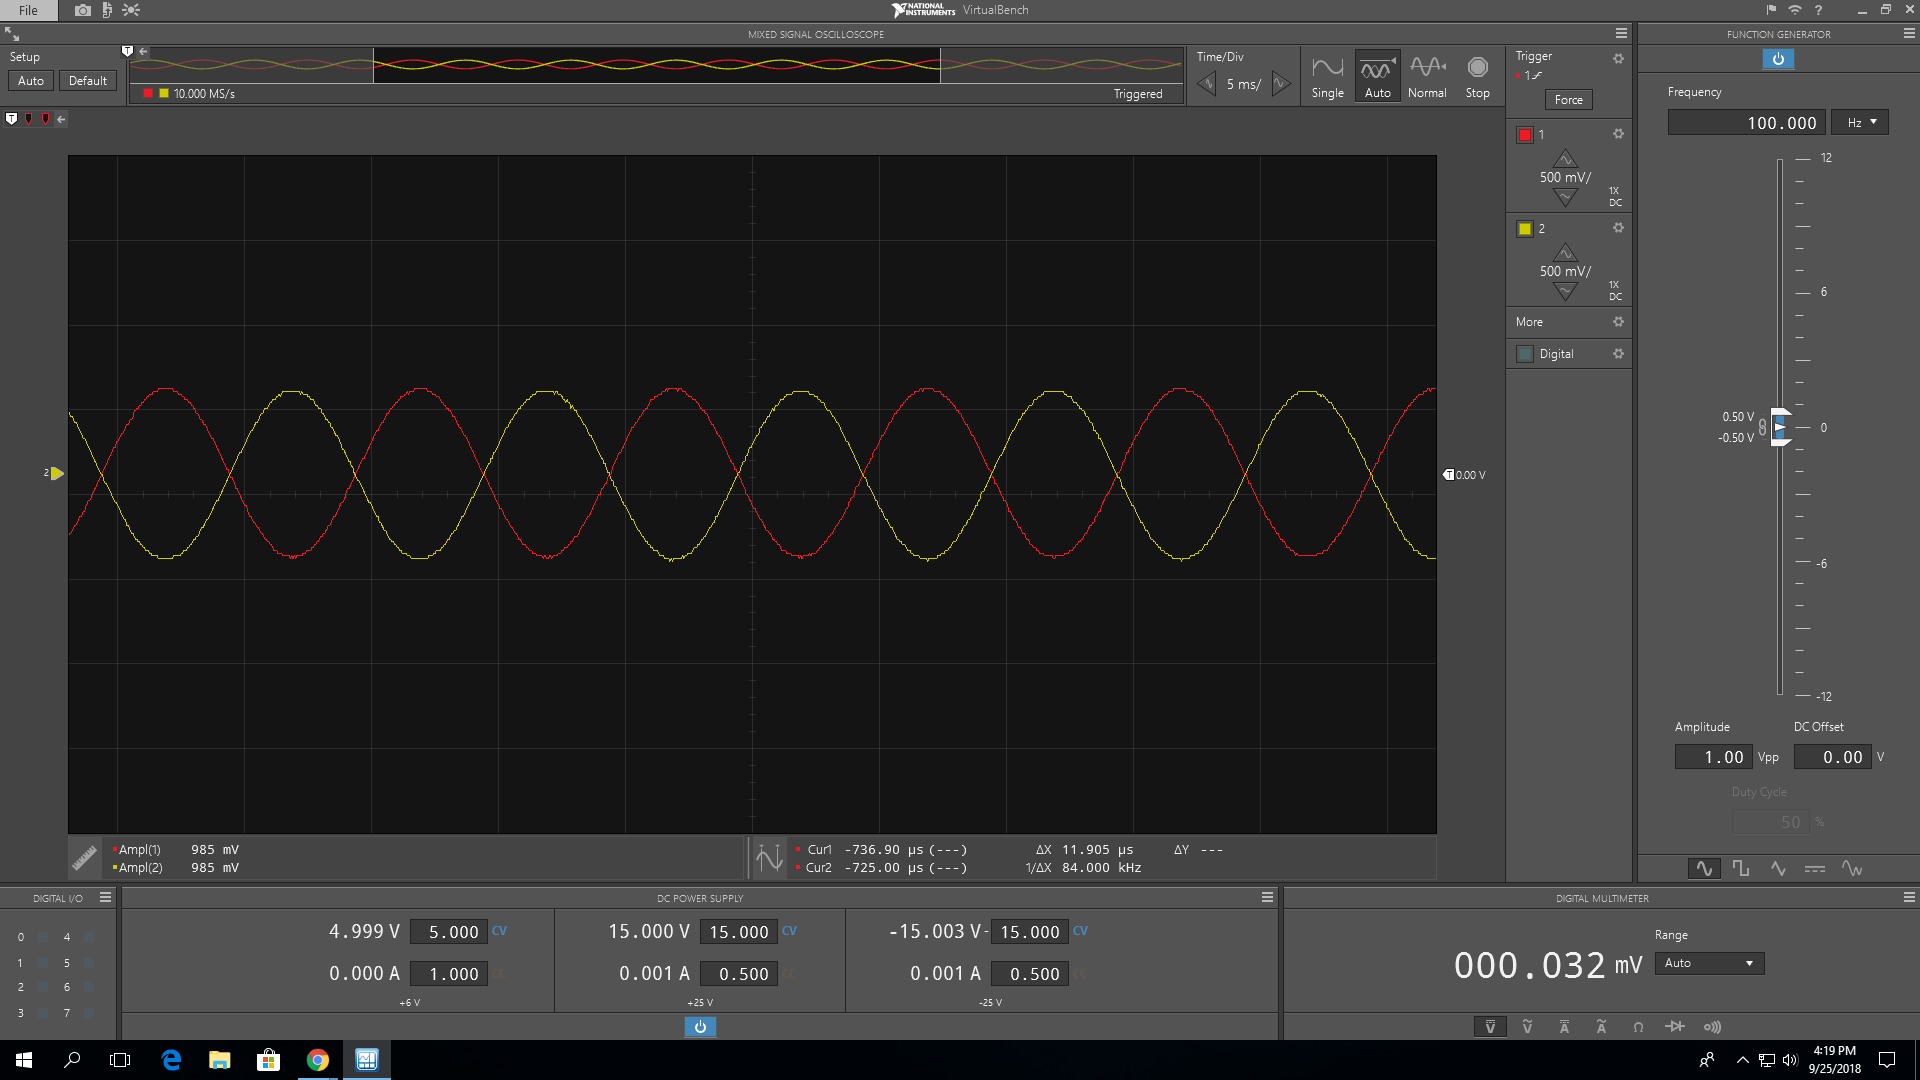
\includegraphics[scale=0.22]{images/invertingamplifier.png}
		\caption{OpAmp Output in Response to 1 $V_{pp}$, 100 Hz sine wave}
	\end{figure}
\end{centering}



\medskip

%\textit{Note (To be deleted): The heart of your report is the presentation of your results and a discussion of those results. In your discussion, you should not only analyze your results, but also discuss the implications of those results.}

\section{References}

Your text here

\medskip

\textit{Note (To be deleted): List any datasheets, websites, lab procedure, etc. used during the lab.}

\section{Conclusion}

Your text here

\medskip

\textit{Note (To be deleted): While the ``Results and Discussion'' section focused on the test results individually, the ``Conclusion'' discusses the results in the context of the entire experiment. Usually, the objectives given in the ``Introduction'' are reviewed to determine whether the experiment succeeded. If the objectives were not met, you should analyze why the results were not as predicted.}

\section{Errors}

Your text here

\medskip

\textit{Note (To be deleted): Briefly list sources of error and discuss how to eliminate or deal with them}

\end{document}
